\scanpage{164}
% position: upper left table
\(\pi'_i\)
\diagram{\(\begin{array}{c|c|c|}
&L_i,&M_i\\\hline
L_i&\chi&\tau_i\\\hline
M_i&0&0\\\hline
\end{array}\)}
\margin{\(\unsure{\prime}\)}
% position: upper middle table
\(\unsure{\varpi'_i|\bar\pi'_i}\)
\figure{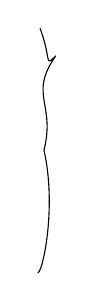
\begin{tikzpicture}
\draw (0,3.1)..controls (.15,2.7) and (.05,2.6)..(.2,2.75)..controls (-.15,2.25) and (.2,2.15)..(.05,1.55)..controls (.22,.8) and (.02,-.05)..(-.03,0);
\end{tikzpicture}}
\diagram{\(\begin{array}{c|c|c}
&L_i&M_i\\\hline
L_i&0&-\tau_i\\\hline
M_i&0&\chi
\end{array}\)}
% position: upper right isolated tensors
\margin{\(\ell_1\otimes m_2\)\par
\((\deleted{\unsure{\ell_1+m_1}}\)}
% position: middle deleted operator
\[
\deleted{\pi'_1\otimes\mathrm{id}_{E_2}+\mathrm{id}_{E_1}\otimes}
\]
% position: middle left empty ruled frame
\figure{\begin{tikzpicture}
\draw (0,2.1)..controls (2,2.3) and (3.1,2.5)..(4.3,2.55);
\draw (.32,2.55)..controls (.3,1.6) and (.55,.7)..(.4,0);
\draw (.36,2.55)--(.36,.55)..controls (.48,.8) and (.45,1)..(.4,1.2);
\end{tikzpicture}}
% position: middle right coefficient table
\diagram{\(\begin{array}{c|ccc}
1&\unsure{\deleted{\mathrm{id}}\inserted{1}}&1&1\\\hline
\pi'_1&\chi&\chi&\tau_1\otimes\mathrm{id}_{L_2}\\[1ex]
\pi'_2&\chi&\mathrm{id}_{L_1}\otimes\tau_2&\chi\\[1ex]
\pi'_1\otimes\pi'_2&\chi^2&\chi\,\mathrm{id}_{L_1}\otimes\tau_2&\chi\tau_1\otimes\mathrm{id}_{L_2}
\end{array}\)}
% position: lower left operator
\[
\alpha+\beta_1\pi'_1+\beta_2\pi'_2+\gamma\pi'_1\otimes\pi'_2
\]
% position: lower left deleted formula
\[
\deleted{\alpha\pi'_1+\beta\pi'}
\]
% position: lower central boxed condition
\[
\deleted{\unsure{\chi}}\quad\boxed{\alpha+(\beta_1+\beta_2)\chi+\gamma\chi^2=\chi}
\]
% position: lower central calculation and bracket
\[
\alpha+\beta_1\chi+
\underbrace{\unsure{\beta_2}\,\mathrm{id}\otimes\tau_2+\gamma\chi\,\mathrm{id}\otimes\tau_2}_{(\beta_2+\gamma\chi)\mathrm{id}\otimes\tau_2}
=\mathrm{id}_{L_1}\otimes\tau_2
\]
% position: bottom left boxed conditions
\[
\boxed{\begin{gathered}
\alpha+\beta_1\chi=0\\
\beta_2+\gamma\chi=1
\end{gathered}}
\]
% position: bottom right marginal expansion
\margin{i.e.\quad\(\begin{gathered}
\mathrm{id}_{L_1}\otimes(\inserted{\alpha+}\unsure{\beta_1}\chi\,\mathrm{id}_{M_2}\\
+(\beta_2+\gamma\chi)\tau_2)=\\
\mathrm{id}\otimes\tau_2
\end{gathered}\)}
% position: foot pencil
\margin{163}
